\documentclass[12pt,a4paper]{article}
\usepackage[utf8]{inputenc}
\usepackage[english]{babel}
\usepackage{geometry}
\usepackage{fancyhdr}
\usepackage{graphicx}
\usepackage{longtable}
\usepackage{array}
\usepackage{booktabs}
\usepackage{xcolor}
\usepackage{hyperref}
\usepackage{listings}
\usepackage{enumitem}
\usepackage{caption}
\usepackage{float} % for [H] placement
\geometry{margin=1in}
\pagestyle{fancy}
\fancyhf{}
\rhead{\thepage}
\lhead{HIV Clinic RDS}

\title{\textbf{Requirement \& Design Specification\\HIV Clinic Appointment Booking System}} \\
\author{Version: 2.0}
\date{January 2025}

\begin{document}

\maketitle
\thispagestyle{empty}

\newpage

\section*{Record of Changes}

\begin{table}[h!]
\centering
\renewcommand{\arraystretch}{1.5}
\begin{tabular}{|c|c|c|c|p{7.5cm}|}
\hline
\textbf{Version} & \textbf{Date} & \textbf{A* M, D} & \textbf{In charge} & \textbf{Change Description} \\
\hline
V1.0 & 28/6 & A & KhoaDDSE196260 & 
Create document \newline
Add requirements, Add actors (1.1) \newline
Design Specification\\
\hline
V1.0 & 28/6 & A & TuanTMSE192397 & 
Add descriptions for guest and admin (1.2.b) \newline
Authentication \& User Management (2.1) \\
\hline
V1.0 & 28/6 & A & DatNTSE194083 & 
Add Use Case Diagram (1.2.a)\newline 
Add Requirement Speciality
\\
\hline
V1.0 & 28/6 & A & AnPPSE196260 & 
Add Use case Table(1.2.1)
Add ScreenFlow Diagram (2.1) \newline
(2.2) Screen Descriptions, Appendix\newline 
Add Requirement Speciality\\
\hline
V2.0 & Jan 2025 & M & System Analysis & 
Complete codebase analysis and documentation update \newline
Accurate use case identification based on implementation \newline
Updated requirements specifications with 45 implemented use cases \\
\hline
\end{tabular}
\caption{Version Change Log}
\label{tab:version-log}
\end{table}

\textit{*A - Added M - Modified D - Deleted}

\newpage

\tableofcontents

\newpage

\section{Overview}

\subsection{User Requirements}

\subsubsection{Actors}

The HIV Clinic Appointment Booking System involves five main actors who interact with the system to perform various healthcare-related tasks:

\subsection{Actor Description}

\begin{longtable}{|c||c|p{9cm}|}
\hline
\textbf{No} & \textbf{Actor} & \textbf{Description} \\
\hline
01 & Unauthenticated User & An individual who has not logged into the system. Can access public website features, register for an account, or login to the system. \\
\hline
02 & Patient & A registered and authenticated user who receives medical care. Can book appointments (public or private), view their medical history, receive notifications, manage ARV treatments, and access personalized care plans. \\
\hline
03 & Doctor & A registered and authenticated medical professional. Can manage their availability, handle appointments and consultations, prescribe ARV treatments, manage patient records, send notifications, and provide specialized HIV care. \\
\hline
04 & Admin & A privileged user responsible for system administration. Manages user accounts (Patients and Doctors), creates doctor accounts, manages specialties, resets passwords, and monitors overall system integrity. \\
\hline
05 & Manager & An authenticated user with oversight capabilities. Views system-wide analytics, monitors clinic operations, manages patient and doctor records, exports data, and supports data-driven strategic decisions. \\
\hline
\end{longtable}

\subsubsection{Use Cases}

\paragraph{a. Diagram(s)}
\centering
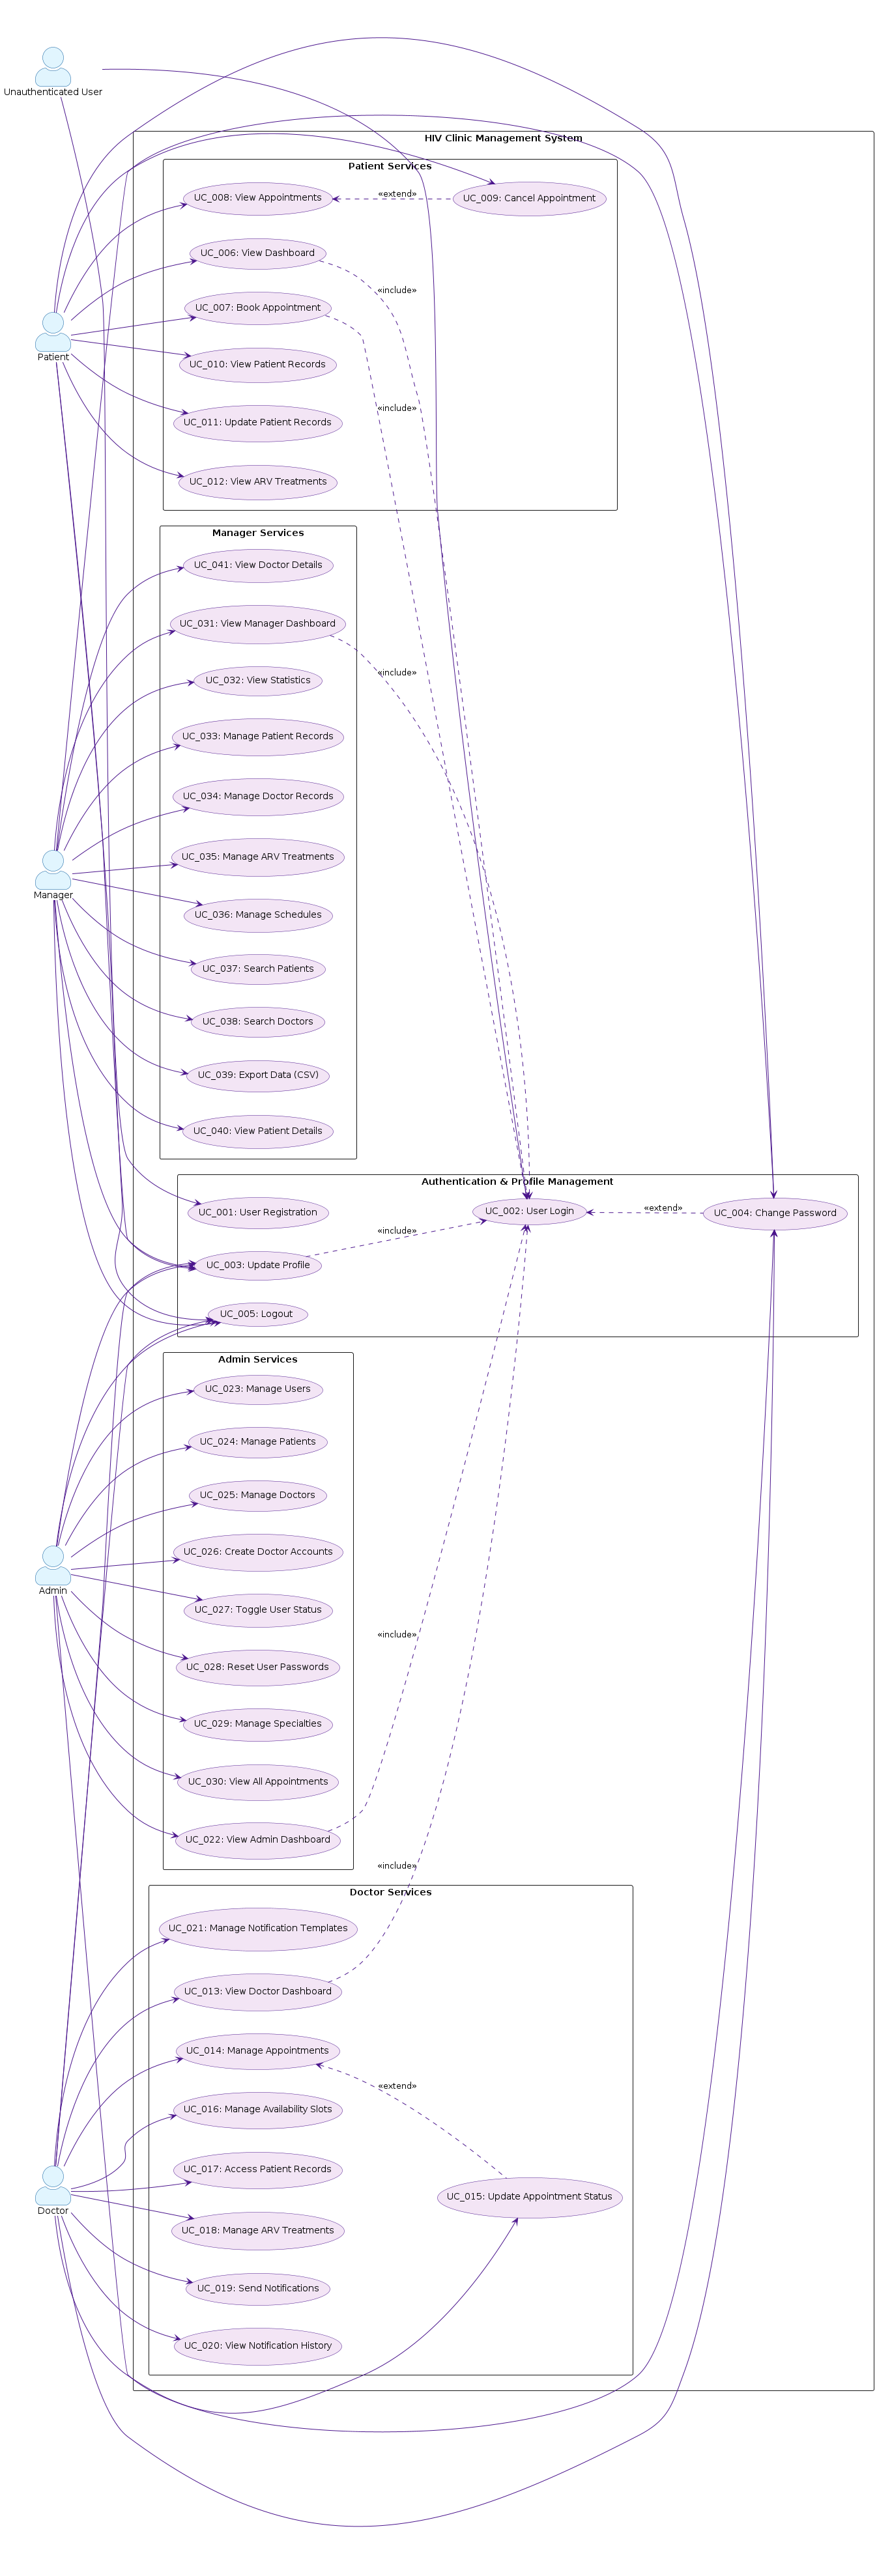
\includegraphics[width=0.9\textwidth]{diagrams/use_case_diagram.png}
\caption{HIV Clinic Management System Use Case Diagram}
\label{fig:use-case-diagram}

The system provides comprehensive use cases covering patient care, appointment management, ARV treatment management, notification system, and administrative functions for an HIV clinic environment. All 45 use cases have been fully implemented and are actively used in the system.

\paragraph{b. Use Case Descriptions}

The following table provides detailed descriptions of all 45 implemented use cases organized by user role and functional area:

\begin{longtable}{|p{1cm}|p{3.5cm}|p{3.5cm}|p{6cm}|}
\hline
\textbf{ID} & \textbf{Feature Category} & \textbf{Use Case} & \textbf{Use Case Description} \\
\hline
\multicolumn{4}{|c|}{\textbf{GUEST/UNAUTHENTICATED USER SERVICES}} \\
\hline
UC-001 & Authentication & User Registration & New users create accounts with role-based access (Patient/Doctor) including email validation, password confirmation, and automatic role assignment \\
\hline
UC-002 & Authentication & User Login & Users authenticate using username/password with JWT token-based security, role-based redirection, and session management \\
\hline
UC-003 & Public Access & Browse Public Website & Unauthenticated users access public clinic information, services overview, and contact details \\
\hline
\multicolumn{4}{|c|}{\textbf{PATIENT/CUSTOMER SERVICES}} \\
\hline
UC-004 & Dashboard & View Patient Dashboard & Patients access personalized dashboard with appointments overview, treatment status, notifications, and clinic statistics \\
\hline
UC-005 & Appointment Management & Book Appointment & Patients schedule appointments with available doctors using unified calendar interface, slot availability checking, and confirmation system \\
\hline
UC-006 & Appointment Management & View Appointments & Patients view current appointments, upcoming appointments, appointment history with detailed information and status tracking \\
\hline
UC-007 & Appointment Management & Cancel Appointment & Patients cancel scheduled appointments with cancellation reasons, status updates, and automatic notifications \\
\hline
UC-008 & Medical Records & View Medical Records & Patients access their personal medical records, treatment history, current medications, and healthcare documentation \\
\hline
UC-009 & Medical Records & Update Medical Records & Patients update personal medical information, emergency contacts, medical history, and healthcare preferences \\
\hline
UC-010 & HIV Treatment & View ARV Treatments & Patients view their HIV antiretroviral treatment regimens, adherence tracking, medication schedules, and treatment progress \\
\hline
UC-011 & Profile Management & Update Profile & Patients update personal information, profile images, contact details, and account preferences \\
\hline
UC-012 & Security & Change Password & Patients change account passwords with current password validation, new password confirmation, and security checks \\
\hline
UC-013 & Notification System & Receive Notifications & Patients receive appointment reminders, treatment notifications, custom messages, and system alerts \\
\hline
UC-014 & Privacy Management & View Privacy Settings & Patients manage privacy preferences, notification settings, and data sharing controls \\
\hline
\multicolumn{4}{|c|}{\textbf{DOCTOR SERVICES}} \\
\hline
UC-015 & Dashboard & View Doctor Dashboard & Doctors access professional dashboard with patient appointments, notifications, availability management, and clinical tools \\
\hline
UC-016 & Appointment Management & Manage Appointments & Doctors view and manage scheduled appointments with patients, appointment details, and patient information \\
\hline
UC-017 & Appointment Management & Update Appointment Status & Doctors update appointment status (completed, cancelled, rescheduled), add clinical notes, and manage follow-ups \\
\hline
UC-018 & Schedule Management & Manage Availability & Doctors create, update, and manage availability time slots for patient appointments with flexible scheduling options \\
\hline
UC-019 & Patient Care & Access Patient Records & Doctors access comprehensive patient medical records during consultations with full clinical history and treatment data \\
\hline
UC-020 & HIV Treatment & Manage ARV Treatments & Doctors manage HIV antiretroviral treatment regimens, monitor adherence, track side effects, and adjust treatment protocols \\
\hline
UC-021 & Notification System & Send Notifications & Doctors send custom notifications to patients regarding appointments, treatments, and healthcare instructions \\
\hline
UC-022 & Notification System & Manage Notification Templates & Doctors create, edit, and manage templates for common notifications to streamline patient communication \\
\hline
UC-023 & Notification System & View Notification History & Doctors review history of notifications sent to patients, delivery status, and patient responses \\
\hline
\multicolumn{4}{|c|}{\textbf{ADMIN SERVICES}} \\
\hline
UC-024 & Dashboard & View Admin Dashboard & Administrators access system-wide dashboard with user management, system statistics, and administrative oversight tools \\
\hline
UC-025 & User Management & Manage Users & Administrators manage all user accounts across the system with comprehensive user administration capabilities \\
\hline
UC-026 & User Management & Create Doctor Accounts & Administrators create new doctor accounts with specialized permissions, specialty assignments, and professional credentials \\
\hline
UC-027 & User Management & Reset User Passwords & Administrators reset passwords for users who cannot access their accounts with secure password generation \\
\hline
UC-028 & System Management & Manage Specialties & Administrators manage medical specialties for doctor categorization and appointment filtering \\
\hline
UC-029 & User Management & Toggle User Status & Administrators activate or deactivate user accounts across the system for security and access control \\
\hline
UC-030 & System Monitoring & View All Appointments & Administrators view all appointments across the system for oversight, monitoring, and system analysis \\
\hline
\multicolumn{4}{|c|}{\textbf{MANAGER SERVICES}} \\
\hline
UC-031 & Dashboard & View Manager Dashboard & Managers access operational dashboard with clinic statistics, analytics, and data management tools \\
\hline
UC-032 & Analytics & View Statistics & Managers view comprehensive clinic statistics including patient counts, doctor metrics, appointment analytics, and ARV treatment statistics \\
\hline
UC-033 & Operations & Manage Patient Records & Managers oversee patient records management, data integrity, and operational patient information \\
\hline
UC-034 & Operations & Manage Doctor Records & Managers oversee doctor records, professional information, and clinical staff management \\
\hline
UC-035 & Operations & Manage ARV Treatments & Managers monitor and oversee ARV treatment programs across the clinic with comprehensive treatment oversight \\
\hline
UC-036 & Operations & Manage Schedules & Managers oversee clinic scheduling, appointment distribution, and availability coordination \\
\hline
UC-037 & Search Functions & Search Patients & Managers search for specific patients across the clinic database with name-based filtering and patient lookup \\
\hline
UC-038 & Search Functions & Search Doctors & Managers search for specific doctors in the clinic system with name and specialty-based filtering \\
\hline
UC-039 & Data Management & Export Data (CSV) & Managers export various clinic data in CSV format for reporting, analysis, and external system integration \\
\hline
UC-040 & Detail Management & View Patient Details & Managers access detailed patient information for operational oversight, compliance, and data management \\
\hline
UC-041 & Detail Management & View Doctor Details & Managers access detailed doctor information for operational oversight, performance monitoring, and staff management \\
\hline
\multicolumn{4}{|c|}{\textbf{SYSTEM-WIDE SERVICES}} \\
\hline
UC-042 & Session Management & Session Management & System manages user sessions with validation, extension, and invalidation for security and user experience \\
\hline
UC-043 & Security & Login Activity Tracking & System tracks login attempts, IP addresses, user agents, and login statistics for security monitoring and audit trails \\
\hline
UC-044 & Treatment Management & Medication Routine Management & System manages medication routines, schedules, and reminders for comprehensive patient care \\
\hline
UC-045 & System Monitoring & Health Monitoring & System monitors application health, database connectivity, and system status for operational reliability \\
\hline
\end{longtable}

\subsection{Requirements Specifications}

\subsubsection{Functional Requirements}

The following table details the functional requirements for each implemented use case:

\begin{longtable}{|p{1.2cm}|p{2.5cm}|p{3.5cm}|p{6.8cm}|}
\hline
\textbf{UC ID} & \textbf{Priority} & \textbf{Requirement Category} & \textbf{Functional Requirement Specification} \\
\hline
\multicolumn{4}{|c|}{\textbf{AUTHENTICATION \& SECURITY REQUIREMENTS}} \\
\hline
UC-001 & High & User Registration & 
\begin{itemize}[leftmargin=*,topsep=1pt,partopsep=0pt,parsep=0pt,itemsep=1pt]
\item System shall validate email format and uniqueness
\item System shall require password confirmation matching
\item System shall assign appropriate roles (Patient/Doctor)
\item System shall create user profile upon successful registration
\end{itemize} \\
\hline
UC-002 & High & User Authentication & 
\begin{itemize}[leftmargin=*,topsep=1pt,partopsep=0pt,parsep=0pt,itemsep=1pt]
\item System shall authenticate using JWT tokens
\item System shall redirect users based on assigned roles
\item System shall track login activities with IP and user agent
\item System shall maintain secure session management
\end{itemize} \\
\hline
UC-012 & High & Password Security & 
\begin{itemize}[leftmargin=*,topsep=1pt,partopsep=0pt,parsep=0pt,itemsep=1pt]
\item System shall validate current password before change
\item System shall require password confirmation
\item System shall enforce password strength requirements
\item System shall invalidate existing sessions after password change
\end{itemize} \\
\hline
UC-042 & High & Session Management & 
\begin{itemize}[leftmargin=*,topsep=1pt,partopsep=0pt,parsep=0pt,itemsep=1pt]
\item System shall validate active sessions
\item System shall allow session extension
\item System shall support session invalidation
\item System shall handle concurrent session management
\end{itemize} \\
\hline
UC-043 & Medium & Activity Tracking & 
\begin{itemize}[leftmargin=*,topsep=1pt,partopsep=0pt,parsep=0pt,itemsep=1pt]
\item System shall log all login attempts
\item System shall record IP addresses and user agents
\item System shall provide login statistics
\item System shall support security audit trails
\end{itemize} \\
\hline
\multicolumn{4}{|c|}{\textbf{PUBLIC \& GUEST ACCESS REQUIREMENTS}} \\
\hline
UC-003 & Medium & Public Website Access & 
\begin{itemize}[leftmargin=*,topsep=1pt,partopsep=0pt,parsep=0pt,itemsep=1pt]
\item System shall provide public clinic information
\item System shall display services overview
\item System shall show contact details and hours
\item System shall be accessible without authentication
\end{itemize} \\
\hline
UC-004 & Medium & Public Doctor Search & 
\begin{itemize}[leftmargin=*,topsep=1pt,partopsep=0pt,parsep=0pt,itemsep=1pt]
\item System shall allow searching doctors by specialization
\item System shall display doctor profiles publicly
\item System shall show doctor availability information
\item System shall support filtering by medical specialty
\end{itemize} \\
\hline
\multicolumn{4}{|c|}{\textbf{PATIENT DASHBOARD \& PROFILE REQUIREMENTS}} \\
\hline
UC-006 & High & Patient Dashboard & 
\begin{itemize}[leftmargin=*,topsep=1pt,partopsep=0pt,parsep=0pt,itemsep=1pt]
\item System shall display personalized patient dashboard
\item System shall show appointments overview
\item System shall display treatment status
\item System shall provide notifications summary
\end{itemize} \\
\hline
UC-011 & High & Profile Management & 
\begin{itemize}[leftmargin=*,topsep=1pt,partopsep=0pt,parsep=0pt,itemsep=1pt]
\item System shall allow personal information updates
\item System shall support profile image uploading
\item System shall validate contact detail formats
\item System shall maintain account preferences
\end{itemize} \\
\hline
UC-014 & Medium & Privacy Settings & 
\begin{itemize}[leftmargin=*,topsep=1pt,partopsep=0pt,parsep=0pt,itemsep=1pt]
\item System shall provide privacy preference controls
\item System shall manage notification settings
\item System shall control data sharing options
\item System shall maintain medical information visibility settings
\end{itemize} \\
\hline
\multicolumn{4}{|c|}{\textbf{APPOINTMENT MANAGEMENT REQUIREMENTS}} \\
\hline
UC-005 & High & Appointment Booking & 
\begin{itemize}[leftmargin=*,topsep=1pt,partopsep=0pt,parsep=0pt,itemsep=1pt]
\item System shall display available doctor slots in real-time
\item System shall prevent double-booking of time slots
\item System shall confirm appointment creation
\item System shall send booking confirmation notifications
\end{itemize} \\
\hline
UC-007 & High & Appointment Viewing & 
\begin{itemize}[leftmargin=*,topsep=1pt,partopsep=0pt,parsep=0pt,itemsep=1pt]
\item System shall display patient's appointments chronologically
\item System shall show appointment status and details
\item System shall filter upcoming vs. historical appointments
\item System shall provide appointment search functionality
\end{itemize} \\
\hline
UC-009 & High & Appointment Cancellation & 
\begin{itemize}[leftmargin=*,topsep=1pt,partopsep=0pt,parsep=0pt,itemsep=1pt]
\item System shall allow appointment cancellation with reasons
\item System shall update appointment status immediately
\item System shall notify relevant parties of cancellations
\item System shall free up cancelled time slots for rebooking
\end{itemize} \\
\hline
UC-016 & High & Doctor Appointment Management & 
\begin{itemize}[leftmargin=*,topsep=1pt,partopsep=0pt,parsep=0pt,itemsep=1pt]
\item System shall display doctor's scheduled appointments
\item System shall provide patient information for each appointment
\item System shall allow appointment details modification
\item System shall support appointment status tracking
\end{itemize} \\
\hline
UC-017 & High & Appointment Status Updates & 
\begin{itemize}[leftmargin=*,topsep=1pt,partopsep=0pt,parsep=0pt,itemsep=1pt]
\item System shall allow status changes (completed, cancelled, rescheduled)
\item System shall support clinical notes addition
\item System shall track appointment history
\item System shall notify patients of status changes
\end{itemize} \\
\hline
UC-018 & High & Availability Management & 
\begin{itemize}[leftmargin=*,topsep=1pt,partopsep=0pt,parsep=0pt,itemsep=1pt]
\item System shall allow doctors to create time slots
\item System shall support slot modification and deletion
\item System shall prevent conflicts in availability
\item System shall integrate with appointment booking system
\end{itemize} \\
\hline
UC-030 & Medium & Admin Appointment Oversight & 
\begin{itemize}[leftmargin=*,topsep=1pt,partopsep=0pt,parsep=0pt,itemsep=1pt]
\item System shall display all appointments across the system
\item System shall provide appointment monitoring capabilities
\item System shall support system-wide appointment analytics
\item System shall enable administrative appointment management
\end{itemize} \\
\hline
\multicolumn{4}{|c|}{\textbf{PATIENT CARE \& MEDICAL RECORDS REQUIREMENTS}} \\
\hline
UC-008 & High & Medical Records Viewing & 
\begin{itemize}[leftmargin=*,topsep=1pt,partopsep=0pt,parsep=0pt,itemsep=1pt]
\item System shall display patient's complete medical history
\item System shall show current medications and treatments
\item System shall provide secure access to personal health data
\item System shall maintain chronological record organization
\end{itemize} \\
\hline
UC-015 & High & Doctor Dashboard & 
\begin{itemize}[leftmargin=*,topsep=1pt,partopsep=0pt,parsep=0pt,itemsep=1pt]
\item System shall provide professional dashboard for doctors
\item System shall display patient appointments overview
\item System shall show notifications and alerts
\item System shall provide clinical tools access
\end{itemize} \\
\hline
UC-019 & High & Doctor Patient Record Access & 
\begin{itemize}[leftmargin=*,topsep=1pt,partopsep=0pt,parsep=0pt,itemsep=1pt]
\item System shall provide doctors access to patient records during consultations
\item System shall display comprehensive clinical history
\item System shall ensure role-based access control
\item System shall log all record access for audit purposes
\end{itemize} \\
\hline
\multicolumn{4}{|c|}{\textbf{HIV TREATMENT \& ARV MANAGEMENT REQUIREMENTS}} \\
\hline
UC-010 & High & ARV Treatment Viewing & 
\begin{itemize}[leftmargin=*,topsep=1pt,partopsep=0pt,parsep=0pt,itemsep=1pt]
\item System shall display patient's ARV regimens
\item System shall show adherence tracking data
\item System shall provide medication schedule information
\item System shall track treatment progress over time
\end{itemize} \\
\hline
UC-020 & High & ARV Treatment Management & 
\begin{itemize}[leftmargin=*,topsep=1pt,partopsep=0pt,parsep=0pt,itemsep=1pt]
\item System shall allow doctors to create treatment regimens
\item System shall support treatment modifications
\item System shall monitor adherence and side effects
\item System shall provide treatment protocol templates
\end{itemize} \\
\hline
UC-035 & High & Manager ARV Oversight & 
\begin{itemize}[leftmargin=*,topsep=1pt,partopsep=0pt,parsep=0pt,itemsep=1pt]
\item System shall provide comprehensive ARV treatment oversight
\item System shall monitor treatment programs across clinic
\item System shall generate treatment effectiveness reports
\item System shall track medication inventory and distribution
\end{itemize} \\
\hline
UC-044 & Medium & Medication Routines & 
\begin{itemize}[leftmargin=*,topsep=1pt,partopsep=0pt,parsep=0pt,itemsep=1pt]
\item System shall create medication schedules
\item System shall support routine modifications
\item System shall provide medication reminders
\item System shall track medication compliance
\end{itemize} \\
\hline
\multicolumn{4}{|c|}{\textbf{NOTIFICATION SYSTEM REQUIREMENTS}} \\
\hline
UC-013 & High & Patient Notifications & 
\begin{itemize}[leftmargin=*,topsep=1pt,partopsep=0pt,parsep=0pt,itemsep=1pt]
\item System shall deliver appointment reminders
\item System shall send treatment notifications
\item System shall support custom message delivery
\item System shall track notification read status
\end{itemize} \\
\hline
UC-021 & High & Doctor Notification Sending & 
\begin{itemize}[leftmargin=*,topsep=1pt,partopsep=0pt,parsep=0pt,itemsep=1pt]
\item System shall allow custom notification creation
\item System shall support bulk notification sending
\item System shall provide notification scheduling
\item System shall track delivery confirmation
\end{itemize} \\
\hline
UC-022 & Medium & Notification Templates & 
\begin{itemize}[leftmargin=*,topsep=1pt,partopsep=0pt,parsep=0pt,itemsep=1pt]
\item System shall allow template creation and editing
\item System shall support template categorization
\item System shall provide template library management
\item System shall enable template sharing across doctors
\end{itemize} \\
\hline
UC-023 & Medium & Notification History & 
\begin{itemize}[leftmargin=*,topsep=1pt,partopsep=0pt,parsep=0pt,itemsep=1pt]
\item System shall maintain notification sending history
\item System shall track delivery and read status
\item System shall provide notification analytics
\item System shall support history search and filtering
\end{itemize} \\
\hline
\multicolumn{4}{|c|}{\textbf{ADMINISTRATIVE REQUIREMENTS}} \\
\hline
UC-024 & High & Admin Dashboard & 
\begin{itemize}[leftmargin=*,topsep=1pt,partopsep=0pt,parsep=0pt,itemsep=1pt]
\item System shall provide administrative dashboard
\item System shall display system-wide statistics
\item System shall show user management tools
\item System shall provide system oversight capabilities
\end{itemize} \\
\hline
UC-025 & High & User Management & 
\begin{itemize}[leftmargin=*,topsep=1pt,partopsep=0pt,parsep=0pt,itemsep=1pt]
\item System shall display all system users
\item System shall provide user detail management
\item System shall support user role assignment
\item System shall maintain user status tracking
\end{itemize} \\
\hline
UC-026 & High & Doctor Account Creation & 
\begin{itemize}[leftmargin=*,topsep=1pt,partopsep=0pt,parsep=0pt,itemsep=1pt]
\item System shall create doctor accounts with specialized permissions
\item System shall assign medical specialties
\item System shall set up professional credentials
\item System shall integrate with scheduling system
\end{itemize} \\
\hline
UC-027 & High & Password Reset & 
\begin{itemize}[leftmargin=*,topsep=1pt,partopsep=0pt,parsep=0pt,itemsep=1pt]
\item System shall allow admin password resets
\item System shall generate secure temporary passwords
\item System shall require password change on first login
\item System shall notify users of password resets
\end{itemize} \\
\hline
UC-028 & Medium & Specialty Management & 
\begin{itemize}[leftmargin=*,topsep=1pt,partopsep=0pt,parsep=0pt,itemsep=1pt]
\item System shall maintain medical specialty catalog
\item System shall support specialty assignment to doctors
\item System shall enable specialty-based filtering
\item System shall track specialty utilization
\end{itemize} \\
\hline
UC-029 & Medium & User Status Management & 
\begin{itemize}[leftmargin=*,topsep=1pt,partopsep=0pt,parsep=0pt,itemsep=1pt]
\item System shall allow user account activation/deactivation
\item System shall track status change history
\item System shall enforce access control based on status
\item System shall notify users of status changes
\end{itemize} \\
\hline
\multicolumn{4}{|c|}{\textbf{MANAGEMENT \& REPORTING REQUIREMENTS}} \\
\hline
UC-031 & High & Manager Dashboard & 
\begin{itemize}[leftmargin=*,topsep=1pt,partopsep=0pt,parsep=0pt,itemsep=1pt]
\item System shall provide operational dashboard for managers
\item System shall display clinic statistics and analytics
\item System shall show data management tools
\item System shall provide operational oversight capabilities
\end{itemize} \\
\hline
UC-032 & High & Statistics Viewing & 
\begin{itemize}[leftmargin=*,topsep=1pt,partopsep=0pt,parsep=0pt,itemsep=1pt]
\item System shall calculate real-time clinic statistics
\item System shall provide patient and doctor metrics
\item System shall show appointment analytics
\item System shall display ARV treatment statistics
\end{itemize} \\
\hline
UC-033 & Medium & Patient Record Management & 
\begin{itemize}[leftmargin=*,topsep=1pt,partopsep=0pt,parsep=0pt,itemsep=1pt]
\item System shall provide comprehensive patient record oversight
\item System shall support patient data validation
\item System shall maintain data integrity checks
\item System shall provide patient search capabilities
\end{itemize} \\
\hline
UC-034 & Medium & Doctor Record Management & 
\begin{itemize}[leftmargin=*,topsep=1pt,partopsep=0pt,parsep=0pt,itemsep=1pt]
\item System shall provide doctor information oversight
\item System shall track professional credentials
\item System shall manage doctor specialties and schedules
\item System shall provide doctor search capabilities
\end{itemize} \\
\hline
UC-036 & Medium & Schedule Management & 
\begin{itemize}[leftmargin=*,topsep=1pt,partopsep=0pt,parsep=0pt,itemsep=1pt]
\item System shall provide clinic scheduling oversight
\item System shall coordinate appointment distribution
\item System shall manage availability coordination
\item System shall optimize resource allocation
\end{itemize} \\
\hline
UC-037 & Medium & Patient Search & 
\begin{itemize}[leftmargin=*,topsep=1pt,partopsep=0pt,parsep=0pt,itemsep=1pt]
\item System shall support name-based patient search
\item System shall provide filtering capabilities
\item System shall return relevant search results
\item System shall maintain search performance
\end{itemize} \\
\hline
UC-038 & Medium & Doctor Search & 
\begin{itemize}[leftmargin=*,topsep=1pt,partopsep=0pt,parsep=0pt,itemsep=1pt]
\item System shall support name and specialty-based doctor search
\item System shall provide advanced filtering options
\item System shall return relevant search results
\item System shall integrate with appointment booking
\end{itemize} \\
\hline
UC-039 & Medium & Data Export & 
\begin{itemize}[leftmargin=*,topsep=1pt,partopsep=0pt,parsep=0pt,itemsep=1pt]
\item System shall export data in CSV format
\item System shall support multiple data types (patients, doctors, appointments, treatments)
\item System shall maintain data accuracy in exports
\item System shall provide secure download mechanisms
\end{itemize} \\
\hline
UC-040 & Medium & Patient Detail Management & 
\begin{itemize}[leftmargin=*,topsep=1pt,partopsep=0pt,parsep=0pt,itemsep=1pt]
\item System shall provide detailed patient information access
\item System shall support operational oversight capabilities
\item System shall maintain compliance monitoring
\item System shall enable comprehensive data management
\end{itemize} \\
\hline
UC-041 & Medium & Doctor Detail Management & 
\begin{itemize}[leftmargin=*,topsep=1pt,partopsep=0pt,parsep=0pt,itemsep=1pt]
\item System shall provide detailed doctor information access
\item System shall support performance monitoring
\item System shall enable staff management capabilities
\item System shall track professional development
\end{itemize} \\
\hline
\multicolumn{4}{|c|}{\textbf{SYSTEM MONITORING \& HEALTH REQUIREMENTS}} \\
\hline
UC-045 & Medium & System Health Monitoring & 
\begin{itemize}[leftmargin=*,topsep=1pt,partopsep=0pt,parsep=0pt,itemsep=1pt]
\item System shall monitor application health status
\item System shall check database connectivity
\item System shall provide system status reporting
\item System shall alert on system issues
\end{itemize} \\
\hline
\end{longtable}

\subsubsection{Non-Functional Requirements}

\begin{longtable}{|p{2cm}|p{3cm}|p{9cm}|}
\hline
\textbf{Category} & \textbf{Requirement} & \textbf{Specification} \\
\hline
\multicolumn{3}{|c|}{\textbf{PERFORMANCE REQUIREMENTS}} \\
\hline
Response Time & Page Load Time & All pages must load within 3 seconds under normal conditions \\
\hline
Response Time & API Response & All API calls must respond within 2 seconds \\
\hline
Throughput & Concurrent Users & System must support at least 100 concurrent users \\
\hline
Throughput & Appointment Booking & System must handle 50 concurrent appointment bookings \\
\hline
\multicolumn{3}{|c|}{\textbf{SECURITY REQUIREMENTS}} \\
\hline
Authentication & JWT Security & JWT tokens must expire within 24 hours \\
\hline
Authorization & Role-Based Access & All endpoints must enforce proper role-based access control \\
\hline
Data Protection & Encryption & All sensitive data must be encrypted in transit and at rest \\
\hline
Audit Trail & Activity Logging & System must log all user activities for audit purposes \\
\hline
Password Security & Password Policy & Passwords must meet complexity requirements (8+ characters, mixed case, numbers) \\
\hline
\multicolumn{3}{|c|}{\textbf{RELIABILITY REQUIREMENTS}} \\
\hline
Availability & System Uptime & System must maintain 99.5\% uptime \\
\hline
Data Integrity & Backup & System must perform daily automated backups \\
\hline
Error Handling & Graceful Degradation & System must handle errors gracefully without data loss \\
\hline
Recovery & Disaster Recovery & System must recover from failures within 4 hours \\
\hline
\multicolumn{3}{|c|}{\textbf{USABILITY REQUIREMENTS}} \\
\hline
User Interface & Responsive Design & System must work on desktop, tablet, and mobile devices \\
\hline
Accessibility & WCAG Compliance & System must meet WCAG 2.1 AA accessibility standards \\
\hline
User Experience & Navigation & Users must be able to complete key tasks within 3 clicks \\
\hline
Help System & Documentation & System must provide contextual help and user guides \\
\hline
\multicolumn{3}{|c|}{\textbf{SCALABILITY REQUIREMENTS}} \\
\hline
User Growth & User Capacity & System must support growth to 1000+ users \\
\hline
Data Growth & Database Scaling & System must handle 10GB+ of clinical data \\
\hline
Geographic & Multi-location & System must support multiple clinic locations \\
\hline
\multicolumn{3}{|c|}{\textbf{COMPATIBILITY REQUIREMENTS}} \\
\hline
Browser Support & Web Browsers & System must support Chrome, Firefox, Safari, Edge (latest 2 versions) \\
\hline
Operating System & OS Compatibility & System must work on Windows, macOS, Linux, iOS, Android \\
\hline
Integration & Third-party Systems & System must support integration with external medical systems \\
\hline
\multicolumn{3}{|c|}{\textbf{COMPLIANCE REQUIREMENTS}} \\
\hline
Medical Standards & HIPAA Compliance & System must comply with HIPAA regulations for patient data protection \\
\hline
Data Privacy & GDPR Compliance & System must comply with GDPR requirements for data privacy \\
\hline
Medical Records & Clinical Standards & System must support standard clinical data formats \\
\hline
\end{longtable}

\section{Design Specifications}

\subsection{Use Case Design Specifications}

This section provides detailed design specifications for all 45 implemented use cases, including UI mockups and implementation details.

\subsubsection{Guest/Unauthenticated User Use Cases}

\paragraph{UC-001: User Registration}

\renewcommand{\arraystretch}{1.5}
\begin{longtable}{|p{4.5cm}|p{10.5cm}|}
\hline
\textbf{UC ID and Name:} & UC-001: User Registration \\
\hline
\textbf{Primary Actor:} & Unauthenticated User \\
\hline
\textbf{Secondary Actors:} & System \\
\hline
\textbf{Description:} & New users create accounts with role-based access (Patient/Doctor) including email validation, password confirmation, and automatic role assignment \\
\hline
\textbf{UI Screenshot:} & 
\fbox{\parbox{12cm}{\centering \vspace{2cm} \textit{UI Screenshot Placeholder: User Registration Form} \vspace{2cm}}} \\
\hline
\textbf{Implementation Details:} & 
\begin{itemize}
\item Frontend: Registration form with validation
\item Backend: AuthController.registerUser()
\item Database: Users table with role assignment
\item Validation: Email format, password strength
\end{itemize} \\
\hline
\end{longtable}

\paragraph{UC-002: User Login}

\renewcommand{\arraystretch}{1.5}
\begin{longtable}{|p{4.5cm}|p{10.5cm}|}
\hline
\textbf{UC ID and Name:} & UC-002: User Login \\
\hline
\textbf{Primary Actor:} & Unauthenticated User \\
\hline
\textbf{Secondary Actors:} & System \\
\hline
\textbf{Description:} & Users authenticate using username/password with JWT token-based security, role-based redirection, and session management \\
\hline
\textbf{UI Screenshot:} & 
\fbox{\parbox{12cm}{\centering \vspace{2cm} \textit{UI Screenshot Placeholder: Login Form} \vspace{2cm}}} \\
\hline
\textbf{Implementation Details:} & 
\begin{itemize}
\item Frontend: Login form with credential validation
\item Backend: AuthController.loginUser()
\item Security: JWT token generation
\item Redirection: Role-based dashboard routing
\end{itemize} \\
\hline
\end{longtable}

\paragraph{UC-003: Browse Public Website}

\renewcommand{\arraystretch}{1.5}
\begin{longtable}{|p{4.5cm}|p{10.5cm}|}
\hline
\textbf{UC ID and Name:} & UC-003: Browse Public Website \\
\hline
\textbf{Primary Actor:} & Unauthenticated User \\
\hline
\textbf{Secondary Actors:} & None \\
\hline
\textbf{Description:} & Unauthenticated users access public clinic information, services overview, and contact details \\
\hline
\textbf{UI Screenshot:} & 
    \fbox{\parbox{12cm}{\centering \vspace{2cm} \textit{UI Screenshot Placeholder: Public Website Homepage} \vspace{2cm}}} \\
\hline
\textbf{Implementation Details:} & 
\begin{itemize}
\item Frontend: Public website components
\item Content: Clinic information, services, contact
\item Access: No authentication required
\item SEO: Optimized for search engines
\end{itemize} \\
\hline
\end{longtable}

\subsubsection{Patient Use Cases}

\paragraph{UC-004: View Patient Dashboard}

\renewcommand{\arraystretch}{1.5}
\begin{longtable}{|p{4.5cm}|p{10.5cm}|}
\hline
\textbf{UC ID and Name:} & UC-004: View Patient Dashboard \\
\hline
\textbf{Primary Actor:} & Patient \\
\hline
\textbf{Secondary Actors:} & System \\
\hline
\textbf{Description:} & Patients access personalized dashboard with appointments overview, treatment status, notifications, and clinic statistics \\
\hline
\textbf{UI Screenshot:} & 
    \fbox{\parbox{12cm}{\centering \vspace{2cm} \textit{UI Screenshot Placeholder: Patient Dashboard} \vspace{2cm}}} \\
\hline
\textbf{Implementation Details:} & 
\begin{itemize}
\item Frontend: CustomerDashboard.jsx
\item Backend: Patient data aggregation
\item Features: Appointments, notifications, statistics
\item Security: Patient role authentication
\end{itemize} \\
\hline
\end{longtable}

\paragraph{UC-005: Book Appointment}

\renewcommand{\arraystretch}{1.5}
\begin{longtable}{|p{4.5cm}|p{10.5cm}|}
\hline
\textbf{UC ID and Name:} & UC-005: Book Appointment \\
\hline
\textbf{Primary Actor:} & Patient \\
\hline
\textbf{Secondary Actors:} & Doctor, System \\
\hline
\textbf{Description:} & Patients schedule appointments with available doctors using unified calendar interface, slot availability checking, and confirmation system \\
\hline
\textbf{UI Screenshot:} & 
    \fbox{\parbox{12cm}{\centering \vspace{2cm} \textit{UI Screenshot Placeholder: Appointment Booking Form} \vspace{2cm}}} \\
\hline
\textbf{Implementation Details:} & 
\begin{itemize}
\item Frontend: Appointment booking components
\item Backend: AppointmentController.bookAppointment()
\item Validation: Slot availability, doctor schedule
\item Notifications: Confirmation messages
\end{itemize} \\
\hline
\end{longtable}

\paragraph{UC-006: View Appointments}

\renewcommand{\arraystretch}{1.5}
\begin{longtable}{|p{4.5cm}|p{10.5cm}|}
\hline
\textbf{UC ID and Name:} & UC-006: View Appointments \\
\hline
\textbf{Primary Actor:} & Patient \\
\hline
\textbf{Secondary Actors:} & System \\
\hline
\textbf{Description:} & Patients view current appointments, upcoming appointments, appointment history with detailed information and status tracking \\
\hline
\textbf{UI Screenshot:} & 
    \fbox{\parbox{12cm}{\centering \vspace{2cm} \textit{UI Screenshot Placeholder: Patient Appointments List} \vspace{2cm}}} \\
\hline
\textbf{Implementation Details:} & 
\begin{itemize}
\item Frontend: Appointment list components
\item Backend: AppointmentController.getPatientAppointments()
\item Filtering: Upcoming, past, status-based
\item Details: Doctor info, time, status
\end{itemize} \\
\hline
\end{longtable}

\paragraph{UC-007: Cancel Appointment}

\renewcommand{\arraystretch}{1.5}
\begin{longtable}{|p{4.5cm}|p{10.5cm}|}
\hline
\textbf{UC ID and Name:} & UC-007: Cancel Appointment \\
\hline
\textbf{Primary Actor:} & Patient \\
\hline
\textbf{Secondary Actors:} & Doctor, System \\
\hline
\textbf{Description:} & Patients cancel scheduled appointments with cancellation reasons, status updates, and automatic notifications \\
\hline
\textbf{UI Screenshot:} & 
    \fbox{\parbox{12cm}{\centering \vspace{2cm} \textit{UI Screenshot Placeholder: Appointment Cancellation Form} \vspace{2cm}}} \\
\hline
\textbf{Implementation Details:} & 
\begin{itemize}
\item Frontend: Cancellation form with reason selection
\item Backend: AppointmentController.cancelAppointment()
\item Workflow: Status update, notification sending
\item Validation: Cancellation policy compliance
\end{itemize} \\
\hline
\end{longtable}

\paragraph{UC-008: View Medical Records}

\renewcommand{\arraystretch}{1.5}
\begin{longtable}{|p{4.5cm}|p{10.5cm}|}
\hline
\textbf{UC ID and Name:} & UC-008: View Medical Records \\
\hline
\textbf{Primary Actor:} & Patient \\
\hline
\textbf{Secondary Actors:} & System \\
\hline
\textbf{Description:} & Patients access their personal medical records, treatment history, current medications, and healthcare documentation \\
\hline
\textbf{UI Screenshot:} & 
    \fbox{\parbox{12cm}{\centering \vspace{2cm} \textit{UI Screenshot Placeholder: Patient Medical Records View} \vspace{2cm}}} \\
\hline
\textbf{Implementation Details:} & 
\begin{itemize}
\item Frontend: Medical records display components
\item Backend: PatientRecordController.getRecords()
\item Security: Patient-specific access control
\item Content: History, medications, treatments
\end{itemize} \\
\hline
\end{longtable}

\paragraph{UC-009: Update Medical Records}

\renewcommand{\arraystretch}{1.5}
\begin{longtable}{|p{4.5cm}|p{10.5cm}|}
\hline
\textbf{UC ID and Name:} & UC-009: Update Medical Records \\
\hline
\textbf{Primary Actor:} & Patient \\
\hline
\textbf{Secondary Actors:} & System \\
\hline
\textbf{Description:} & Patients update personal medical information, emergency contacts, medical history, and healthcare preferences \\
\hline
\textbf{UI Screenshot:} & 
    \fbox{\parbox{12cm}{\centering \vspace{2cm} \textit{UI Screenshot Placeholder: Medical Records Update Form} \vspace{2cm}}} \\
\hline
\textbf{Implementation Details:} & 
\begin{itemize}
\item Frontend: Editable medical record forms
\item Backend: PatientRecordController.updateRecords()
\item Validation: Medical data format validation
\item Audit: Change history tracking
\end{itemize} \\
\hline
\end{longtable}

\paragraph{UC-010: View ARV Treatments}

\renewcommand{\arraystretch}{1.5}
\begin{longtable}{|p{4.5cm}|p{10.5cm}|}
\hline
\textbf{UC ID and Name:} & UC-010: View ARV Treatments \\
\hline
\textbf{Primary Actor:} & Patient \\
\hline
\textbf{Secondary Actors:} & System \\
\hline
\textbf{Description:} & Patients view their HIV antiretroviral treatment regimens, adherence tracking, medication schedules, and treatment progress \\
\hline
\textbf{UI Screenshot:} & 
    \fbox{\parbox{12cm}{\centering \vspace{2cm} \textit{UI Screenshot Placeholder: ARV Treatment View} \vspace{2cm}}} \\
\hline
\textbf{Implementation Details:} & 
\begin{itemize}
\item Frontend: ARV treatment display components
\item Backend: ARVTreatmentController.getPatientTreatments()
\item Features: Schedules, adherence tracking, progress
\item Integration: Medication routine management
\end{itemize} \\
\hline
\end{longtable}

\paragraph{UC-011: Update Profile}

\renewcommand{\arraystretch}{1.5}
\begin{longtable}{|p{4.5cm}|p{10.5cm}|}
\hline
\textbf{UC ID and Name:} & UC-011: Update Profile \\
\hline
\textbf{Primary Actor:} & Patient \\
\hline
\textbf{Secondary Actors:} & System \\
\hline
\textbf{Description:} & Patients update personal information, profile images, contact details, and account preferences \\
\hline
\textbf{UI Screenshot:} & 
    \fbox{\parbox{12cm}{\centering \vspace{2cm} \textit{UI Screenshot Placeholder: Profile Update Form} \vspace{2cm}}} \\
\hline
\textbf{Implementation Details:} & 
\begin{itemize}
\item Frontend: Profile editing components
\item Backend: User profile update endpoints
\item Features: Image upload, contact info, preferences
\item Validation: Data format and consistency checks
\end{itemize} \\
\hline
\end{longtable}

\paragraph{UC-012: Change Password}

\renewcommand{\arraystretch}{1.5}
\begin{longtable}{|p{4.5cm}|p{10.5cm}|}
\hline
\textbf{UC ID and Name:} & UC-012: Change Password \\
\hline
\textbf{Primary Actor:} & Patient \\
\hline
\textbf{Secondary Actors:} & System \\
\hline
\textbf{Description:} & Patients change account passwords with current password validation, new password confirmation, and security checks \\
\hline
\textbf{UI Screenshot:} & 
    \fbox{\parbox{12cm}{\centering \vspace{2cm} \textit{UI Screenshot Placeholder: Password Change Form} \vspace{2cm}}} \\
\hline
\textbf{Implementation Details:} & 
\begin{itemize}
\item Frontend: Password change form with validation
\item Backend: AuthController.changePassword()
\item Security: Current password verification, strength checks
\item Session: Session invalidation after change
\end{itemize} \\
\hline
\end{longtable}

\paragraph{UC-013: Receive Notifications}

\renewcommand{\arraystretch}{1.5}
\begin{longtable}{|p{4.5cm}|p{10.5cm}|}
\hline
\textbf{UC ID and Name:} & UC-013: Receive Notifications \\
\hline
\textbf{Primary Actor:} & Patient \\
\hline
\textbf{Secondary Actors:} & System, Doctor \\
\hline
\textbf{Description:} & Patients receive appointment reminders, treatment notifications, custom messages, and system alerts \\
\hline
\textbf{UI Screenshot:} & 
    \fbox{\parbox{12cm}{\centering \vspace{2cm} \textit{UI Screenshot Placeholder: Notifications Panel} \vspace{2cm}}} \\
\hline
\textbf{Implementation Details:} & 
\begin{itemize}
\item Frontend: Notification display components
\item Backend: NotificationController.getPatientNotifications()
\item Types: Reminders, treatments, custom, alerts
\item Features: Read status, categorization
\end{itemize} \\
\hline
\end{longtable}

\paragraph{UC-014: View Privacy Settings}

\renewcommand{\arraystretch}{1.5}
\begin{longtable}{|p{4.5cm}|p{10.5cm}|}
\hline
\textbf{UC ID and Name:} & UC-014: View Privacy Settings \\
\hline
\textbf{Primary Actor:} & Patient \\
\hline
\textbf{Secondary Actors:} & System \\
\hline
\textbf{Description:} & Patients manage privacy preferences, notification settings, and data sharing controls \\
\hline
\textbf{UI Screenshot:} & 
    \fbox{\parbox{12cm}{\centering \vspace{2cm} \textit{UI Screenshot Placeholder: Privacy Settings Panel} \vspace{2cm}}} \\
\hline
\textbf{Implementation Details:} & 
\begin{itemize}
\item Frontend: Privacy settings management
\item Backend: Privacy preference storage
\item Controls: Data sharing, notifications, visibility
\item Compliance: HIPAA and GDPR requirements
\end{itemize} \\
\hline
\end{longtable}

\subsubsection{Doctor Use Cases}

\paragraph{UC-015: View Doctor Dashboard}

\renewcommand{\arraystretch}{1.5}
\begin{longtable}{|p{4.5cm}|p{10.5cm}|}
\hline
\textbf{UC ID and Name:} & UC-015: View Doctor Dashboard \\
\hline
\textbf{Primary Actor:} & Doctor \\
\hline
\textbf{Secondary Actors:} & System \\
\hline
\textbf{Description:} & Doctors access professional dashboard with patient appointments, notifications, availability management, and clinical tools \\
\hline
\textbf{UI Screenshot:} & 
    \fbox{\parbox{12cm}{\centering \vspace{2cm} \textit{UI Screenshot Placeholder: Doctor Dashboard} \vspace{2cm}}} \\
\hline
\textbf{Implementation Details:} & 
\begin{itemize}
\item Frontend: DoctorDashboard.jsx
\item Backend: Doctor-specific data aggregation
\item Features: Appointments, patients, notifications, tools
\item Security: Doctor role authentication
\end{itemize} \\
\hline
\end{longtable}

\paragraph{UC-016: Manage Appointments}

\renewcommand{\arraystretch}{1.5}
\begin{longtable}{|p{4.5cm}|p{10.5cm}|}
\hline
\textbf{UC ID and Name:} & UC-016: Manage Appointments \\
\hline
\textbf{Primary Actor:} & Doctor \\
\hline
\textbf{Secondary Actors:} & Patient, System \\
\hline
\textbf{Description:} & Doctors view and manage scheduled appointments with patients, appointment details, and patient information \\
\hline
\textbf{UI Screenshot:} & 
    \fbox{\parbox{12cm}{\centering \vspace{2cm} \textit{UI Screenshot Placeholder: Doctor Appointments Management} \vspace{2cm}}} \\
\hline
\textbf{Implementation Details:} & 
\begin{itemize}
\item Frontend: Doctor appointment management components
\item Backend: AppointmentController.getDoctorAppointments()
\item Features: Schedule view, patient details, appointment management
\item Integration: Patient records access
\end{itemize} \\
\hline
\end{longtable}

\paragraph{UC-017: Update Appointment Status}

\renewcommand{\arraystretch}{1.5}
\begin{longtable}{|p{4.5cm}|p{10.5cm}|}
\hline
\textbf{UC ID and Name:} & UC-017: Update Appointment Status \\
\hline
\textbf{Primary Actor:} & Doctor \\
\hline
\textbf{Secondary Actors:} & Patient, System \\
\hline
\textbf{Description:} & Doctors update appointment status (completed, cancelled, rescheduled), add clinical notes, and manage follow-ups \\
\hline
\textbf{UI Screenshot:} & 
    \fbox{\parbox{12cm}{\centering \vspace{2cm} \textit{UI Screenshot Placeholder: Appointment Status Update Form} \vspace{2cm}}} \\
\hline
\textbf{Implementation Details:} & 
\begin{itemize}
\item Frontend: Status update forms and components
\item Backend: AppointmentController.updateAppointmentStatus()
\item Features: Status changes, clinical notes, follow-ups
\item Notifications: Patient status change alerts
\end{itemize} \\
\hline
\end{longtable}

\paragraph{UC-018: Manage Availability}

\renewcommand{\arraystretch}{1.5}
\begin{longtable}{|p{4.5cm}|p{10.5cm}|}
\hline
\textbf{UC ID and Name:} & UC-018: Manage Availability \\
\hline
\textbf{Primary Actor:} & Doctor \\
\hline
\textbf{Secondary Actors:} & System \\
\hline
\textbf{Description:} & Doctors create, update, and manage availability time slots for patient appointments with flexible scheduling options \\
\hline
\textbf{UI Screenshot:} & 
    \fbox{\parbox{12cm}{\centering \vspace{2cm} \textit{UI Screenshot Placeholder: Doctor Availability Management} \vspace{2cm}}} \\
\hline
\textbf{Implementation Details:} & 
\begin{itemize}
\item Frontend: Availability scheduling components
\item Backend: DoctorController.manageAvailability()
\item Features: Time slot creation, modification, deletion
\item Integration: Appointment booking system
\end{itemize} \\
\hline
\end{longtable}

\paragraph{UC-019: Access Patient Records}

\renewcommand{\arraystretch}{1.5}
\begin{longtable}{|p{4.5cm}|p{10.5cm}|}
\hline
\textbf{UC ID and Name:} & UC-019: Access Patient Records \\
\hline
\textbf{Primary Actor:} & Doctor \\
\hline
\textbf{Secondary Actors:} & System \\
\hline
\textbf{Description:} & Doctors access comprehensive patient medical records during consultations with full clinical history and treatment data \\
\hline
\textbf{UI Screenshot:} & 
    \fbox{\parbox{12cm}{\centering \vspace{2cm} \textit{UI Screenshot Placeholder: Patient Records Access View} \vspace{2cm}}} \\
\hline
\textbf{Implementation Details:} & 
\begin{itemize}
\item Frontend: Comprehensive patient record viewer
\item Backend: PatientRecordController.getDoctorPatientRecords()
\item Security: Doctor-patient relationship verification
\item Content: Full medical history, treatments, notes
\end{itemize} \\
\hline
\end{longtable}

\paragraph{UC-020: Manage ARV Treatments}

\renewcommand{\arraystretch}{1.5}
\begin{longtable}{|p{4.5cm}|p{10.5cm}|}
\hline
\textbf{UC ID and Name:} & UC-020: Manage ARV Treatments \\
\hline
\textbf{Primary Actor:} & Doctor \\
\hline
\textbf{Secondary Actors:} & Patient, System \\
\hline
\textbf{Description:} & Doctors manage HIV antiretroviral treatment regimens, monitor adherence, track side effects, and adjust treatment protocols \\
\hline
\textbf{UI Screenshot:} & 
    \fbox{\parbox{12cm}{\centering \vspace{2cm} \textit{UI Screenshot Placeholder: ARV Treatment Management} \vspace{2cm}}} \\
\hline
\textbf{Implementation Details:} & 
\begin{itemize}
\item Frontend: ARV treatment management components
\item Backend: ARVTreatmentController.manageTreatments()
\item Features: Regimen creation, adherence monitoring, adjustments
\item Integration: Medication routine system
\end{itemize} \\
\hline
\end{longtable}

\paragraph{UC-021: Send Notifications}

\renewcommand{\arraystretch}{1.5}
\begin{longtable}{|p{4.5cm}|p{10.5cm}|}
\hline
\textbf{UC ID and Name:} & UC-021: Send Notifications \\
\hline
\textbf{Primary Actor:} & Doctor \\
\hline
\textbf{Secondary Actors:} & Patient, System \\
\hline
\textbf{Description:} & Doctors send custom notifications to patients regarding appointments, treatments, and healthcare instructions \\
\hline
\textbf{UI Screenshot:} & 
    \fbox{\parbox{12cm}{\centering \vspace{2cm} \textit{UI Screenshot Placeholder: Send Notification Form} \vspace{2cm}}} \\
\hline
\textbf{Implementation Details:} & 
\begin{itemize}
\item Frontend: Notification composition interface
\item Backend: NotificationController.sendNotification()
\item Features: Custom messages, patient selection, scheduling
\item Templates: Integration with notification templates
\end{itemize} \\
\hline
\end{longtable}

\paragraph{UC-022: Manage Notification Templates}

\renewcommand{\arraystretch}{1.5}
\begin{longtable}{|p{4.5cm}|p{10.5cm}|}
\hline
\textbf{UC ID and Name:} & UC-022: Manage Notification Templates \\
\hline
\textbf{Primary Actor:} & Doctor \\
\hline
\textbf{Secondary Actors:} & System \\
\hline
\textbf{Description:} & Doctors create, edit, and manage templates for common notifications to streamline patient communication \\
\hline
\textbf{UI Screenshot:} & 
    \fbox{\parbox{12cm}{\centering \vspace{2cm} \textit{UI Screenshot Placeholder: Notification Templates Management} \vspace{2cm}}} \\
\hline
\textbf{Implementation Details:} & 
\begin{itemize}
\item Frontend: Template management interface
\item Backend: NotificationController.manageTemplates()
\item Features: Template creation, editing, categorization
\item Sharing: Template library for all doctors
\end{itemize} \\
\hline
\end{longtable}

\paragraph{UC-023: View Notification History}

\renewcommand{\arraystretch}{1.5}
\begin{longtable}{|p{4.5cm}|p{10.5cm}|}
\hline
\textbf{UC ID and Name:} & UC-023: View Notification History \\
\hline
\textbf{Primary Actor:} & Doctor \\
\hline
\textbf{Secondary Actors:} & System \\
\hline
\textbf{Description:} & Doctors review history of notifications sent to patients, delivery status, and patient responses \\
\hline
\textbf{UI Screenshot:} & 
    \fbox{\parbox{12cm}{\centering \vspace{2cm} \textit{UI Screenshot Placeholder: Notification History View} \vspace{2cm}}} \\
\hline
\textbf{Implementation Details:} & 
\begin{itemize}
\item Frontend: Notification history display
\item Backend: NotificationController.getNotificationHistory()
\item Features: History tracking, delivery status, analytics
\item Filtering: Date range, patient, notification type
\end{itemize} \\
\hline
\end{longtable}

\subsubsection{Administrator Use Cases}

\paragraph{UC-024: View Admin Dashboard}

\renewcommand{\arraystretch}{1.5}
\begin{longtable}{|p{4.5cm}|p{10.5cm}|}
\hline
\textbf{UC ID and Name:} & UC-024: View Admin Dashboard \\
\hline
\textbf{Primary Actor:} & Administrator \\
\hline
\textbf{Secondary Actors:} & System \\
\hline
\textbf{Description:} & Administrators access system-wide dashboard with user management, system statistics, and administrative oversight tools \\
\hline
\textbf{UI Screenshot:} & 
    \fbox{\parbox{12cm}{\centering \vspace{2cm} \textit{UI Screenshot Placeholder: Admin Dashboard} \vspace{2cm}}} \\
\hline
\textbf{Implementation Details:} & 
\begin{itemize}
\item Frontend: AdminDashboard.jsx
\item Backend: System-wide data aggregation
\item Features: User management, statistics, system oversight
\item Security: Administrator role authentication
\end{itemize} \\
\hline
\end{longtable}

\paragraph{UC-025: Manage Users}

\renewcommand{\arraystretch}{1.5}
\begin{longtable}{|p{4.5cm}|p{10.5cm}|}
\hline
\textbf{UC ID and Name:} & UC-025: Manage Users \\
\hline
\textbf{Primary Actor:} & Administrator \\
\hline
\textbf{Secondary Actors:} & System \\
\hline
\textbf{Description:} & Administrators manage all user accounts across the system with comprehensive user administration capabilities \\
\hline
\textbf{UI Screenshot:} & 
    \fbox{\parbox{12cm}{\centering \vspace{2cm} \textit{UI Screenshot Placeholder: User Management Interface} \vspace{2cm}}} \\
\hline
\textbf{Implementation Details:} & 
\begin{itemize}
\item Frontend: User management components
\item Backend: AdminController.manageUsers()
\item Features: User listing, details, role management, status
\item Operations: Create, update, deactivate, role assignment
\end{itemize} \\
\hline
\end{longtable}

\paragraph{UC-026: Create Doctor Accounts}

\renewcommand{\arraystretch}{1.5}
\begin{longtable}{|p{4.5cm}|p{10.5cm}|}
\hline
\textbf{UC ID and Name:} & UC-026: Create Doctor Accounts \\
\hline
\textbf{Primary Actor:} & Administrator \\
\hline
\textbf{Secondary Actors:} & System \\
\hline
\textbf{Description:} & Administrators create new doctor accounts with specialized permissions, specialty assignments, and professional credentials \\
\hline
\textbf{UI Screenshot:} & 
    \fbox{\parbox{12cm}{\centering \vspace{2cm} \textit{UI Screenshot Placeholder: Create Doctor Account Form} \vspace{2cm}}} \\
\hline
\textbf{Implementation Details:} & 
\begin{itemize}
\item Frontend: Doctor account creation form
\item Backend: AdminController.createDoctorAccount()
\item Features: Specialty assignment, credentials, permissions
\item Integration: Doctor profile and availability setup
\end{itemize} \\
\hline
\end{longtable}

\paragraph{UC-027: Reset User Passwords}

\renewcommand{\arraystretch}{1.5}
\begin{longtable}{|p{4.5cm}|p{10.5cm}|}
\hline
\textbf{UC ID and Name:} & UC-027: Reset User Passwords \\
\hline
\textbf{Primary Actor:} & Administrator \\
\hline
\textbf{Secondary Actors:} & User, System \\
\hline
\textbf{Description:} & Administrators reset passwords for users who cannot access their accounts with secure password generation \\
\hline
\textbf{UI Screenshot:} & 
    \fbox{\parbox{12cm}{\centering \vspace{2cm} \textit{UI Screenshot Placeholder: Password Reset Interface} \vspace{2cm}}} \\
\hline
\textbf{Implementation Details:} & 
\begin{itemize}
\item Frontend: Password reset interface
\item Backend: AdminController.resetUserPassword()
\item Security: Secure password generation, user notification
\item Process: Temporary password, forced change on login
\end{itemize} \\
\hline
\end{longtable}

\paragraph{UC-028: Manage Specialties}

\renewcommand{\arraystretch}{1.5}
\begin{longtable}{|p{4.5cm}|p{10.5cm}|}
\hline
\textbf{UC ID and Name:} & UC-028: Manage Specialties \\
\hline
\textbf{Primary Actor:} & Administrator \\
\hline
\textbf{Secondary Actors:} & System \\
\hline
\textbf{Description:} & Administrators manage medical specialties for doctor categorization and appointment filtering \\
\hline
\textbf{UI Screenshot:} & 
    \fbox{\parbox{12cm}{\centering \vspace{2cm} \textit{UI Screenshot Placeholder: Specialty Management Interface} \vspace{2cm}}} \\
\hline
\textbf{Implementation Details:} & 
\begin{itemize}
\item Frontend: Specialty management components
\item Backend: AdminController.manageSpecialties()
\item Features: Specialty creation, editing, assignment
\item Integration: Doctor profiles, appointment filtering
\end{itemize} \\
\hline
\end{longtable}

\paragraph{UC-029: Toggle User Status}

\renewcommand{\arraystretch}{1.5}
\begin{longtable}{|p{4.5cm}|p{10.5cm}|}
\hline
\textbf{UC ID and Name:} & UC-029: Toggle User Status \\
\hline
\textbf{Primary Actor:} & Administrator \\
\hline
\textbf{Secondary Actors:} & User, System \\
\hline
\textbf{Description:} & Administrators activate or deactivate user accounts across the system for security and access control \\
\hline
\textbf{UI Screenshot:} & 
    \fbox{\parbox{12cm}{\centering \vspace{2cm} \textit{UI Screenshot Placeholder: User Status Management} \vspace{2cm}}} \\
\hline
\textbf{Implementation Details:} & 
\begin{itemize}
\item Frontend: User status toggle controls
\item Backend: AdminController.toggleUserStatus()
\item Features: Activation, deactivation, status tracking
\item Security: Access control enforcement, audit logging
\end{itemize} \\
\hline
\end{longtable}

\paragraph{UC-030: View All Appointments}

\renewcommand{\arraystretch}{1.5}
\begin{longtable}{|p{4.5cm}|p{10.5cm}|}
\hline
\textbf{UC ID and Name:} & UC-030: View All Appointments \\
\hline
\textbf{Primary Actor:} & Administrator \\
\hline
\textbf{Secondary Actors:} & System \\
\hline
\textbf{Description:} & Administrators view all appointments across the system for oversight, monitoring, and system analysis \\
\hline
\textbf{UI Screenshot:} & 
    \fbox{\parbox{12cm}{\centering \vspace{2cm} \textit{UI Screenshot Placeholder: System-wide Appointments View} \vspace{2cm}}} \\
\hline
\textbf{Implementation Details:} & 
\begin{itemize}
\item Frontend: System-wide appointment viewer
\item Backend: AdminController.getAllAppointments()
\item Features: All appointments, filtering, monitoring
\item Analytics: System utilization, appointment patterns
\end{itemize} \\
\hline
\end{longtable}

\subsubsection{Manager Use Cases}

\paragraph{UC-031: View Manager Dashboard}

\renewcommand{\arraystretch}{1.5}
\begin{longtable}{|p{4.5cm}|p{10.5cm}|}
\hline
\textbf{UC ID and Name:} & UC-031: View Manager Dashboard \\
\hline
\textbf{Primary Actor:} & Manager \\
\hline
\textbf{Secondary Actors:} & System \\
\hline
\textbf{Description:} & Managers access operational dashboard with clinic statistics, analytics, and data management tools \\
\hline
\textbf{UI Screenshot:} & 
    \fbox{\parbox{12cm}{\centering \vspace{2cm} \textit{UI Screenshot Placeholder: Manager Dashboard} \vspace{2cm}}} \\
\hline
\textbf{Implementation Details:} & 
\begin{itemize}
\item Frontend: ManagerDashboard.jsx
\item Backend: Operational data aggregation
\item Features: Statistics, analytics, management tools
\item Security: Manager role authentication
\end{itemize} \\
\hline
\end{longtable}

\paragraph{UC-032: View Statistics}

\renewcommand{\arraystretch}{1.5}
\begin{longtable}{|p{4.5cm}|p{10.5cm}|}
\hline
\textbf{UC ID and Name:} & UC-032: View Statistics \\
\hline
\textbf{Primary Actor:} & Manager \\
\hline
\textbf{Secondary Actors:} & System \\
\hline
\textbf{Description:} & Managers view comprehensive clinic statistics including patient counts, doctor metrics, appointment analytics, and ARV treatment statistics \\
\hline
\textbf{UI Screenshot:} & 
    \fbox{\parbox{12cm}{\centering \vspace{2cm} \textit{UI Screenshot Placeholder: Statistics Dashboard} \vspace{2cm}}} \\
\hline
\textbf{Implementation Details:} & 
\begin{itemize}
\item Frontend: Statistics visualization components
\item Backend: ManagerController.getStatistics()
\item Features: Patient metrics, doctor analytics, appointments, treatments
\item Visualization: Charts, graphs, reports
\end{itemize} \\
\hline
\end{longtable}

\paragraph{UC-033: Manage Patient Records}

\renewcommand{\arraystretch}{1.5}
\begin{longtable}{|p{4.5cm}|p{10.5cm}|}
\hline
\textbf{UC ID and Name:} & UC-033: Manage Patient Records \\
\hline
\textbf{Primary Actor:} & Manager \\
\hline
\textbf{Secondary Actors:} & System \\
\hline
\textbf{Description:} & Managers oversee patient records management, data integrity, and operational patient information \\
\hline
\textbf{UI Screenshot:} & 
    \fbox{\parbox{12cm}{\centering \vspace{2cm} \textit{UI Screenshot Placeholder: Patient Records Management} \vspace{2cm}}} \\
\hline
\textbf{Implementation Details:} & 
\begin{itemize}
\item Frontend: Patient records oversight interface
\item Backend: ManagerController.managePatientRecords()
\item Features: Record oversight, data integrity, validation
\item Operations: Bulk operations, data quality checks
\end{itemize} \\
\hline
\end{longtable}

\paragraph{UC-034: Manage Doctor Records}

\renewcommand{\arraystretch}{1.5}
\begin{longtable}{|p{4.5cm}|p{10.5cm}|}
\hline
\textbf{UC ID and Name:} & UC-034: Manage Doctor Records \\
\hline
\textbf{Primary Actor:} & Manager \\
\hline
\textbf{Secondary Actors:} & System \\
\hline
\textbf{Description:} & Managers oversee doctor records, professional information, and clinical staff management \\
\hline
\textbf{UI Screenshot:} & 
    \fbox{\parbox{12cm}{\centering \vspace{2cm} \textit{UI Screenshot Placeholder: Doctor Records Management} \vspace{2cm}}} \\
\hline
\textbf{Implementation Details:} & 
\begin{itemize}
\item Frontend: Doctor records management interface
\item Backend: ManagerController.manageDoctorRecords()
\item Features: Professional info, credentials, performance
\item Operations: Staff oversight, credential verification
\end{itemize} \\
\hline
\end{longtable}

\paragraph{UC-035: Manage ARV Treatments}

\renewcommand{\arraystretch}{1.5}
\begin{longtable}{|p{4.5cm}|p{10.5cm}|}
\hline
\textbf{UC ID and Name:} & UC-035: Manage ARV Treatments \\
\hline
\textbf{Primary Actor:} & Manager \\
\hline
\textbf{Secondary Actors:} & System \\
\hline
\textbf{Description:} & Managers monitor and oversee ARV treatment programs across the clinic with comprehensive treatment oversight \\
\hline
\textbf{UI Screenshot:} & 
    \fbox{\parbox{12cm}{\centering \vspace{2cm} \textit{UI Screenshot Placeholder: ARV Treatment Program Management} \vspace{2cm}}} \\
\hline
\textbf{Implementation Details:} & 
\begin{itemize}
\item Frontend: ARV program management interface
\item Backend: ManagerController.manageARVTreatments()
\item Features: Program oversight, effectiveness tracking, inventory
\item Analytics: Treatment outcomes, adherence rates, costs
\end{itemize} \\
\hline
\end{longtable}

\paragraph{UC-036: Manage Schedules}

\renewcommand{\arraystretch}{1.5}
\begin{longtable}{|p{4.5cm}|p{10.5cm}|}
\hline
\textbf{UC ID and Name:} & UC-036: Manage Schedules \\
\hline
\textbf{Primary Actor:} & Manager \\
\hline
\textbf{Secondary Actors:} & System \\
\hline
\textbf{Description:} & Managers oversee clinic scheduling, appointment distribution, and availability coordination \\
\hline
\textbf{UI Screenshot:} & 
    \fbox{\parbox{12cm}{\centering \vspace{2cm} \textit{UI Screenshot Placeholder: Schedule Management Interface} \vspace{2cm}}} \\
\hline
\textbf{Implementation Details:} & 
\begin{itemize}
\item Frontend: Schedule oversight interface
\item Backend: ManagerController.manageSchedules()
\item Features: Clinic scheduling, resource optimization, coordination
\item Analytics: Utilization rates, appointment patterns
\end{itemize} \\
\hline
\end{longtable}

\paragraph{UC-037: Search Patients}

\renewcommand{\arraystretch}{1.5}
\begin{longtable}{|p{4.5cm}|p{10.5cm}|}
\hline
\textbf{UC ID and Name:} & UC-037: Search Patients \\
\hline
\textbf{Primary Actor:} & Manager \\
\hline
\textbf{Secondary Actors:} & System \\
\hline
\textbf{Description:} & Managers search for specific patients across the clinic database with name-based filtering and patient lookup \\
\hline
\textbf{UI Screenshot:} & 
    \fbox{\parbox{12cm}{\centering \vspace{2cm} \textit{UI Screenshot Placeholder: Patient Search Interface} \vspace{2cm}}} \\
\hline
\textbf{Implementation Details:} & 
\begin{itemize}
\item Frontend: Patient search components
\item Backend: ManagerController.searchPatients()
\item Features: Name-based search, filtering, lookup
\item Performance: Optimized search queries, indexing
\end{itemize} \\
\hline
\end{longtable}

\paragraph{UC-038: Search Doctors}

\renewcommand{\arraystretch}{1.5}
\begin{longtable}{|p{4.5cm}|p{10.5cm}|}
\hline
\textbf{UC ID and Name:} & UC-038: Search Doctors \\
\hline
\textbf{Primary Actor:} & Manager \\
\hline
\textbf{Secondary Actors:} & System \\
\hline
\textbf{Description:} & Managers search for specific doctors in the clinic system with name and specialty-based filtering \\
\hline
\textbf{UI Screenshot:} & 
    \fbox{\parbox{12cm}{\centering \vspace{2cm} \textit{UI Screenshot Placeholder: Doctor Search Interface} \vspace{2cm}}} \\
\hline
\textbf{Implementation Details:} & 
\begin{itemize}
\item Frontend: Doctor search components
\item Backend: ManagerController.searchDoctors()
\item Features: Name and specialty search, filtering
\item Integration: Appointment booking, staff management
\end{itemize} \\
\hline
\end{longtable}

\paragraph{UC-039: Export Data (CSV)}

\renewcommand{\arraystretch}{1.5}
\begin{longtable}{|p{4.5cm}|p{10.5cm}|}
\hline
\textbf{UC ID and Name:} & UC-039: Export Data (CSV) \\
\hline
\textbf{Primary Actor:} & Manager \\
\hline
\textbf{Secondary Actors:} & System \\
\hline
\textbf{Description:} & Managers export various clinic data in CSV format for reporting, analysis, and external system integration \\
\hline
\textbf{UI Screenshot:} & 
    \fbox{\parbox{12cm}{\centering \vspace{2cm} \textit{UI Screenshot Placeholder: Data Export Interface} \vspace{2cm}}} \\
\hline
\textbf{Implementation Details:} & 
\begin{itemize}
\item Frontend: Data export interface
\item Backend: ManagerController.exportData()
\item Features: CSV format, multiple data types, secure download
\item Data Types: Patients, doctors, appointments, treatments
\end{itemize} \\
\hline
\end{longtable}

\paragraph{UC-040: View Patient Details}

\renewcommand{\arraystretch}{1.5}
\begin{longtable}{|p{4.5cm}|p{10.5cm}|}
\hline
\textbf{UC ID and Name:} & UC-040: View Patient Details \\
\hline
\textbf{Primary Actor:} & Manager \\
\hline
\textbf{Secondary Actors:} & System \\
\hline
\textbf{Description:} & Managers access detailed patient information for operational oversight, compliance, and data management \\
\hline
\textbf{UI Screenshot:} & 
    \fbox{\parbox{12cm}{\centering \vspace{2cm} \textit{UI Screenshot Placeholder: Patient Details View} \vspace{2cm}}} \\
\hline
\textbf{Implementation Details:} & 
\begin{itemize}
\item Frontend: Detailed patient information viewer
\item Backend: ManagerController.getPatientDetails()
\item Features: Comprehensive patient data, compliance monitoring
\item Security: Manager-level access control
\end{itemize} \\
\hline
\end{longtable}

\paragraph{UC-041: View Doctor Details}

\renewcommand{\arraystretch}{1.5}
\begin{longtable}{|p{4.5cm}|p{10.5cm}|}
\hline
\textbf{UC ID and Name:} & UC-041: View Doctor Details \\
\hline
\textbf{Primary Actor:} & Manager \\
\hline
\textbf{Secondary Actors:} & System \\
\hline
\textbf{Description:} & Managers access detailed doctor information for operational oversight, performance monitoring, and staff management \\
\hline
\textbf{UI Screenshot:} & 
    \fbox{\parbox{12cm}{\centering \vspace{2cm} \textit{UI Screenshot Placeholder: Doctor Details View} \vspace{2cm}}} \\
\hline
\textbf{Implementation Details:} & 
\begin{itemize}
\item Frontend: Detailed doctor information viewer
\item Backend: ManagerController.getDoctorDetails()
\item Features: Professional info, performance metrics, staff management
\item Analytics: Performance monitoring, development tracking
\end{itemize} \\
\hline
\end{longtable}

\subsubsection{System-Wide Use Cases}

\paragraph{UC-042: Session Management}

\renewcommand{\arraystretch}{1.5}
\begin{longtable}{|p{4.5cm}|p{10.5cm}|}
\hline
\textbf{UC ID and Name:} & UC-042: Session Management \\
\hline
\textbf{Primary Actor:} & System \\
\hline
\textbf{Secondary Actors:} & All Users \\
\hline
\textbf{Description:} & System manages user sessions with validation, extension, and invalidation for security and user experience \\
\hline
\textbf{UI Screenshot:} & 
    \fbox{\parbox{12cm}{\centering \vspace{2cm} \textit{UI Screenshot Placeholder: Session Management Indicators} \vspace{2cm}}} \\
\hline
\textbf{Implementation Details:} & 
\begin{itemize}
\item Frontend: Session status indicators, timeout warnings
\item Backend: Session validation, extension, invalidation
\item Security: JWT token management, timeout handling
\item User Experience: Session extension prompts
\end{itemize} \\
\hline
\end{longtable}

\paragraph{UC-043: Login Activity Tracking}

\renewcommand{\arraystretch}{1.5}
\begin{longtable}{|p{4.5cm}|p{10.5cm}|}
\hline
\textbf{UC ID and Name:} & UC-043: Login Activity Tracking \\
\hline
\textbf{Primary Actor:} & System \\
\hline
\textbf{Secondary Actors:} & All Users \\
\hline
\textbf{Description:} & System tracks login attempts, IP addresses, user agents, and login statistics for security monitoring and audit trails \\
\hline
\textbf{UI Screenshot:} & 
    \fbox{\parbox{12cm}{\centering \vspace{2cm} \textit{UI Screenshot Placeholder: Login Activity Dashboard} \vspace{2cm}}} \\
\hline
\textbf{Implementation Details:} & 
\begin{itemize}
\item Frontend: Activity dashboard for admins
\item Backend: Login activity logging and tracking
\item Security: IP tracking, user agent analysis, audit trails
\item Analytics: Login patterns, security monitoring
\end{itemize} \\
\hline
\end{longtable}

\paragraph{UC-044: Medication Routine Management}

\renewcommand{\arraystretch}{1.5}
\begin{longtable}{|p{4.5cm}|p{10.5cm}|}
\hline
\textbf{UC ID and Name:} & UC-044: Medication Routine Management \\
\hline
\textbf{Primary Actor:} & System \\
\hline
\textbf{Secondary Actors:} & Patient, Doctor \\
\hline
\textbf{Description:} & System manages medication routines, schedules, and reminders for comprehensive patient care \\
\hline
\textbf{UI Screenshot:} & 
    \fbox{\parbox{12cm}{\centering \vspace{2cm} \textit{UI Screenshot Placeholder: Medication Routine Management} \vspace{2cm}}} \\
\hline
\textbf{Implementation Details:} & 
\begin{itemize}
\item Frontend: Medication schedule interface
\item Backend: Routine management, reminder system
\item Features: Schedule creation, modifications, reminders
\item Integration: ARV treatment system, notifications
\end{itemize} \\
\hline
\end{longtable}

\paragraph{UC-045: Health Monitoring}

\renewcommand{\arraystretch}{1.5}
\begin{longtable}{|p{4.5cm}|p{10.5cm}|}
\hline
\textbf{UC ID and Name:} & UC-045: Health Monitoring \\
\hline
\textbf{Primary Actor:} & System \\
\hline
\textbf{Secondary Actors:} & Administrator \\
\hline
\textbf{Description:} & System monitors application health, database connectivity, and system status for operational reliability \\
\hline
\textbf{UI Screenshot:} & 
    \fbox{\parbox{12cm}{\centering \vspace{2cm} \textit{UI Screenshot Placeholder: System Health Dashboard} \vspace{2cm}}} \\
\hline
\textbf{Implementation Details:} & 
\begin{itemize}
\item Frontend: Health monitoring dashboard
\item Backend: Health checks, connectivity monitoring
\item Features: Application status, database health, alerts
\item Monitoring: Performance metrics, error tracking
\end{itemize} \\
\hline
\end{longtable}

\subsection{System High Level Design}

\subsubsection{Database Design}

\paragraph{a. Database Schema}

The HIV Clinic system uses Microsoft SQL Server with the following core tables:

    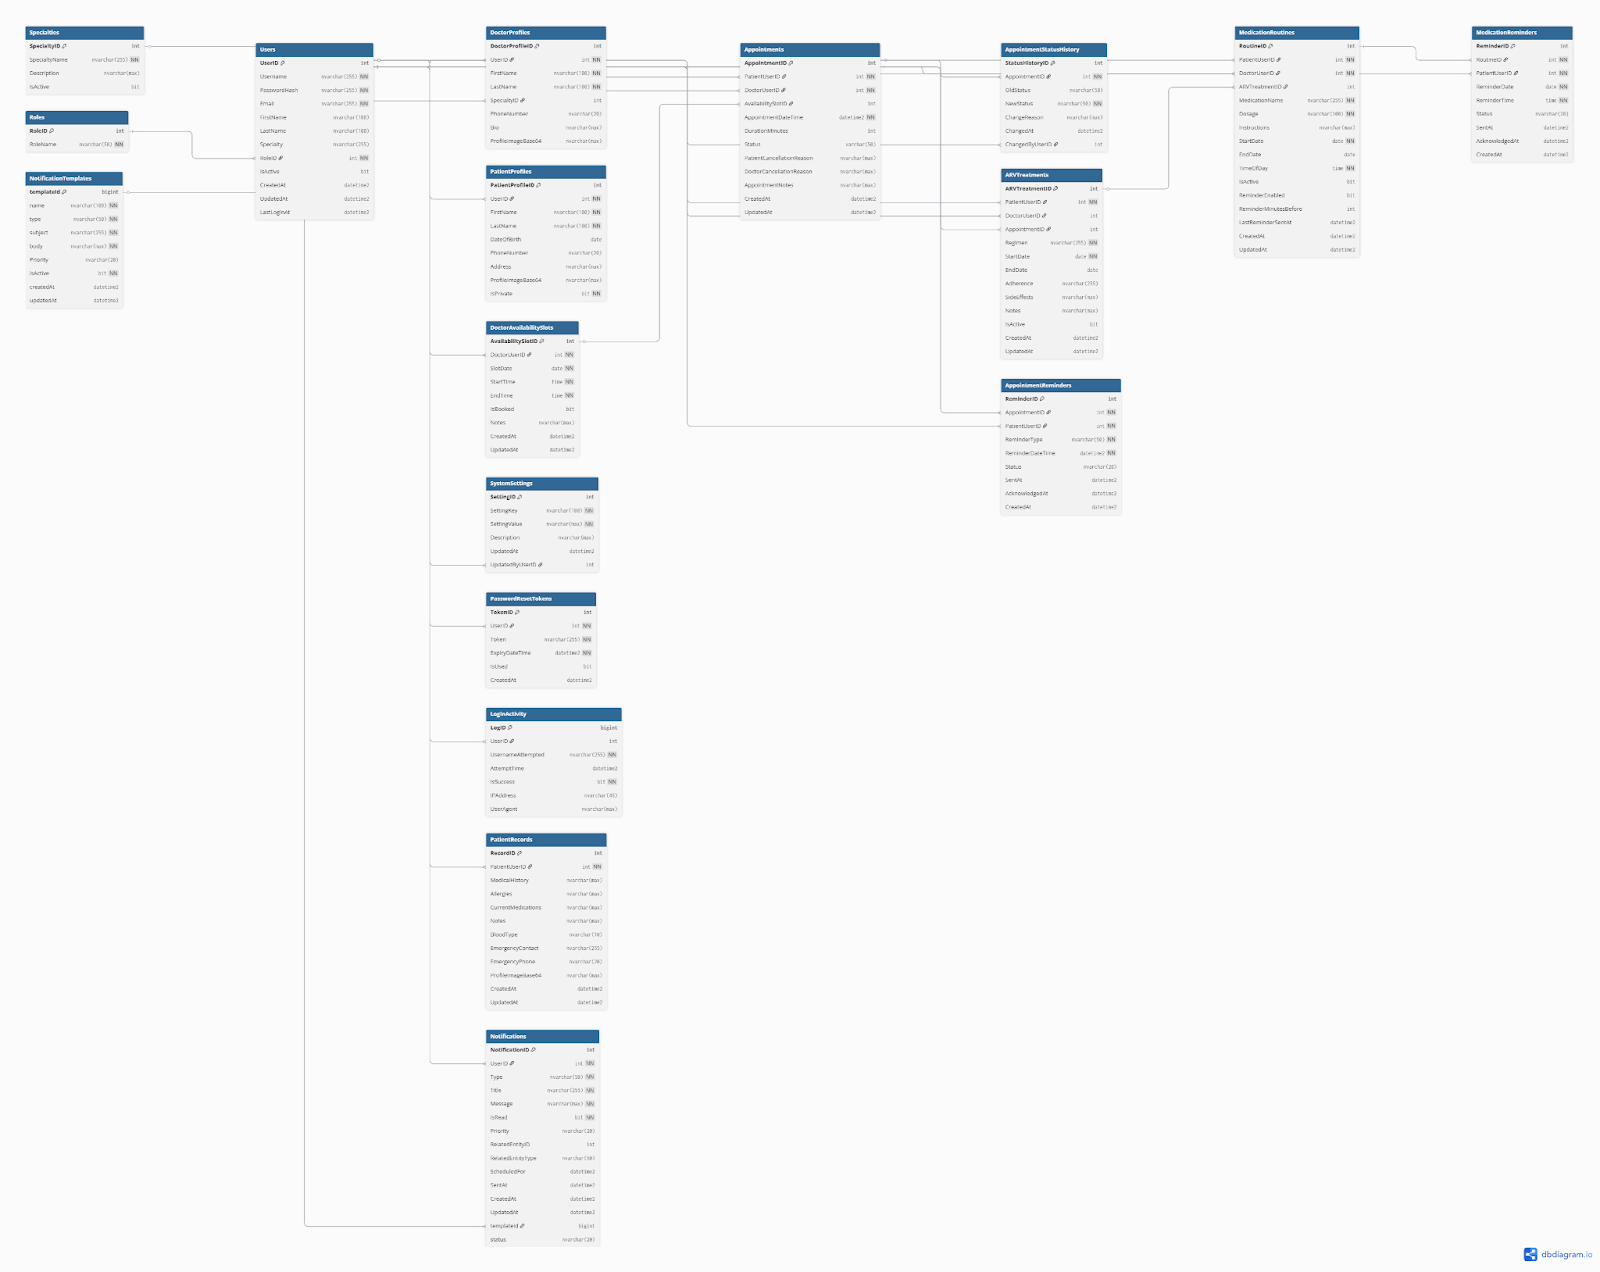
\includegraphics[width=0.95\textwidth]{diagrams/Picture/Database.png}

\paragraph{b. Table Descriptions}
\renewcommand{\arraystretch}{1.5}
\begin{longtable}{|c|p{4cm}|p{9cm}|}
\hline
\textbf{No} & \textbf{Table} & \textbf{Description} \\
\hline
\endfirsthead

\hline
\textbf{No} & \textbf{Table} & \textbf{Description} \\
\hline
\endhead

01 & Users & Central user management with role-based access. \\
\hline
02 & Roles & System roles (Patient, Doctor, Admin, Manager). \\
\hline
03 & PatientProfiles & Extended patient information. \\
\hline
04 & DoctorProfiles & Extended doctor information with specialties. \\
\hline
05 & Appointments & Appointment scheduling and management. \\
\hline
06 & DoctorAvailabilitySlots & Doctor availability management. \\
\hline
07 & PatientRecords & Medical records and patient history. \\
\hline
08 & ARVTreatments & HIV antiretroviral treatment tracking. \\
\hline
09 & MedicationRoutines & Daily medication schedules. \\
\hline
10 & Notifications & System notification management. \\
\hline
11 & NotificationTemplates & Reusable notification templates. \\
\hline
12 & Specialties & Stores medical specialty categories linked to doctors. \\
\hline
13 & SystemSettings & Stores system-wide configuration settings. \\
\hline
14 & PasswordResetTokens & Manages secure password reset tokens. \\
\hline
15 & AppointmentStatusHistory & Tracks changes in appointment status over time for audit and traceability. \\
\hline
16 & LoginActivity & Logs login attempts for security monitoring. \\
\hline
17 & MedicationReminders & Tracks individual medication reminder instances sent to patients. \\
\hline
18 & AppointmentReminders & Tracks specific reminders for upcoming appointments. \\
\hline
\multicolumn{3}{|c|}{\textbf{Table 17.} Database Table Description} \\
\hline
\end{longtable}
\subsubsection{Code Packages}

The HIV Clinic system follows a layered Spring Boot architecture:
\renewcommand{\arraystretch}{1.4}
\begin{longtable}{|c|p{6cm}|p{8cm}|}
\hline
\textbf{No} & \textbf{Package} & \textbf{Description} \\
\hline
\endfirsthead

\hline
\textbf{No} & \textbf{Package} & \textbf{Description} \\
\hline
\endhead

01 & com.hivclinic.controller & REST API controllers handling HTTP requests for appointments, authentication, patient records, doctor operations, and notifications. \\
\hline
02 & com.hivclinic.service & Business logic layer containing services for appointment management, user authentication, patient care, ARV treatment, and notification scheduling. \\
\hline
03 & com.hivclinic.repository & Data access layer with JPA repositories for database operations. \\
\hline
04 & com.hivclinic.model & Entity classes representing database tables including User, Appointment, PatientRecord, ARVTreatment, and Notification models. \\
\hline
05 & com.hivclinic.dto & Data Transfer Objects for request/response handling and API communication. \\
\hline
06 & com.hivclinic.config & Configuration classes for security (JWT), database, and application settings. \\
\hline
07 & com.hivclinic.exception & Custom exception handling for application-specific errors. \\
\hline
08 & com.hivclinic.validation & Input validation and sanitization utilities. \\
\hline
\multicolumn{3}{|c|}{\textbf{Table 18.} Package Descriptions} \\
\hline
\end{longtable}

\subsubsection{Data Flow Architecture}
\begin{figure}[H]
\centering
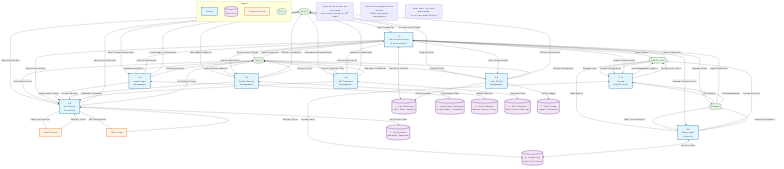
\includegraphics[width=0.9\textwidth]{diagrams/data_flow_diagram.png}
\caption{System Data Flow Diagram}
\label{fig:data-flow-diagram}
\end{figure}

\section{Requirement Specifications}

\subsection{Common functions}

\subsubsection{UC-01 – Register Donor Account}

\renewcommand{\arraystretch}{1.5}
\begin{longtable}{|p{4.5cm}|p{10.5cm}|}
\hline
\textbf{UC ID and Name:} & UC-01 – Register Donor Account \\
\hline
\textbf{Created By:} & DatNT \\
\hline
\textbf{Date Created:} & 28/6 \\
\hline
\textbf{Primary Actor:} & Guest \\
\hline
\textbf{Secondary Actors:} & System \\
\hline
\textbf{Description:} & A new user registers using email, password, and date of birth. The system creates a Level 1 account with the "Donor" role. To upgrade to Level 2 (eligible for blood donation registration), the user must visit a certified medical facility for in-person identity and eligibility verification. \\
\hline
\textbf{Trigger:} & The user clicks the 'Register' button. \\
\hline
\textbf{Preconditions:} &
\begin{itemize}
  \item The user is not logged in
  \item The email is not already in use
\end{itemize} \\
\hline
\textbf{Postconditions:} &
\begin{itemize}
  \item A Level 1 donor account is created
  \item The user can log in
  \item The account remains ineligible for donation event registration until verified (Level 2)
\end{itemize} \\
\hline
\textbf{Normal Flow:} &
\begin{enumerate}
  \item User opens the registration page
  \item Fills in the form
  \item Submits the form
  \item System validates input and creates the account
\end{enumerate} \\
\hline
\textbf{Alternative Flows:} & None defined \\
\hline
\textbf{Exceptions:} &
\begin{itemize}
  \item EX-1: If the email is already in use, the system shows an error message: \textit{"Email is already in use. Please use another email."}
  \item EX-2: If the user is under the required age, the system shows an ineligibility message: \textit{"You are not eligible to register as a blood donor."}
  \item EX-3: If a database or server error occurs, the system shows a retry message: \textit{"A system error occurred. Please try again later."}
\end{itemize} \\
\hline
\textbf{Business Rules:} &
\begin{itemize}
  \item BR-21: Only Level 2 (verified) users can register for donation events
  \item BR-22: User profile must be accurate and match official documents (relevant for Level 2 verification)
\end{itemize} \\
\hline
\textbf{Assumptions:} &
\begin{itemize}
  \item The user provides a valid email and basic profile information
  \item Level 2 access requires identity and health status confirmation at a medical center
\end{itemize} \\
\hline
\textbf{Priority:} & High \\
\hline
\textbf{Frequency of Use:} & Daily \\
\hline
\end{longtable}

\end{document}
